\documentclass[11pt,a4paper]{article}
\usepackage[latin1]{inputenc}
\usepackage{amsmath,amsfonts,amssymb,amsthm,bm}
\usepackage[no-weekday]{eukdate}
\usepackage{graphicx,color,hyperref}
\usepackage{fullpage,parskip,setspace,paralist}
\usepackage{sidecap}
\usepackage[section]{placeins}

\usepackage[style=authoryear-comp, natbib=true]{biblatex}
\ExecuteBibliographyOptions{bibencoding=utf8,minnames=1,maxnames=3,
maxbibnames=99,dashed=false,terseinits=true,giveninits=true,uniquename=false,
uniquelist=false,doi=false, isbn=false,url=true,sortcites=false}
\DeclareFieldFormat[article]{volume}{\mkbibbold{#1}}
\DeclareFieldFormat[article]{number}{\mkbibparens{#1}}
\DeclareFieldFormat[article]{pages}{#1}
\DeclareFieldFormat[article]{title}{\MakeCapital{#1}}
\usepackage{xpatch}
\xpatchbibmacro{volume+number+eid}{\setunit*{\adddot}}{}{}{}
\renewbibmacro{in:}{%
  \ifentrytype{article}{}{%
  \printtext{\bibstring{in}\intitlepunct}}}

\bibliography{fda}

\newtheorem{definition} {Definition}[section]
\newtheorem{lemma} {Lemma}[section]
\newtheorem{Example} {Example}[section]
\newtheorem{Theorem} {Theorem}[section]
\newtheorem{Proposition} {Proposition}[section]
\newtheorem{Corollary}{Corollary}[section]
\newtheorem{Note}{Note}[section]
\numberwithin{equation}{section}

\allowdisplaybreaks
\newcommand{\E}{\mathbb{E}}
\widowpenalty=10000
\clubpenalty=10000
\setcounter{topnumber}{2}
\setcounter{bottomnumber}{2}
\setcounter{totalnumber}{4}
\renewcommand{\topfraction}{0.85}
\renewcommand{\bottomfraction}{0.85}
\renewcommand{\textfraction}{0.15}
\renewcommand{\floatpagefraction}{0.7}


\begin{document}

\title{Seasonal functional autoregressive models}
\author{Atefeh Zamani, ??, Rob J Hyndman}
\maketitle

\begin{abstract}
  Functional autoregressive models are popular for functional time series analysis, but they fail to address seasonal behaviour in functional time series data. To overcome this shortcoming, we introduce seasonal functional autoregressive time series models. For the model of order one, we derive sufficient stationarity conditions and limiting behavior, and provide estimation and prediction methods. Some properties of the general order $P$ model are also presented. The merits of these models are demonstrated using simulation studies and via an application to real data.
\end{abstract}

\emph{Keywords}:
  Functional time series analysis, seasonal functional autoregressive model, central limit theorem, prediction, estimation.

\onehalfspacing

%****************************************************************************************************************************

\section{Introduction}\label{sec:intro}

Improved acquisition techniques make it possible to collect a large amount of high-dimensional data, including data that can be considered functional \citep{ramsay1982data}. Functional time series arise when such data are collected over time. We are interested in functional time series which exhibit seasonality. The underlying functional process is denoted by $f_t(x)$, where $t=1,\dots,T$ indexes regularly spaced time and $x$ is a continuous variable.

A seasonal pattern exists when $f_t(x)$ is influenced by seasonal factors (e.g., the quarter of the year, the month, the day of the week, etc.). Usually seasonality is considered to be of fixed and known period and we say that a (possibly de-trended series) is seasonal if its expected value varies in a periodic pattern. Specifically, if
$$
  \E(f_{t}(x)) = \E(f_{t+S}(x)),
$$
we say that the series has seasonality of period $S$.

For example, consider satellite observations measuring the normalized difference vegetation index (NDVI) \citep{he2018statistical}. These are often averaged to obtain monthly observations over the land surface. Here $x$ denotes the two spatial dimensions, while $t$ denotes the month. Seasonal patterns are present due to the natural annual patterns of vegetation variation.

Another example arises in demography where $f_t(x)$ is the mortality rate for people aged $x$ at time $t$ \citep{HU07}. When such data are collected more frequently than annually, seasonality arises due to deaths being influenced by weather.

In other applications, $x$ may denote a second time variable. For example, \citet{hormann2018testing} study pollution data observed every 30 minutes. The long time series is sliced into separate functions, where $x$ denotes the time of day, and $t$ denotes the day. A similar approach has been applied to the
 El Nino-Southern Oscillation (ENSO) (\citet{besse2000autoregressive}), Eurodollar futures rates (\citet{Kargin2008} and \citet{horvath2013estimation}), electricity demand (\citet{shang2013functional}), and many other applications.

Although, the term ``functional data analysis'' was coined by \citet{ramsay1982data}, the history of this area is much older and dates back to \citet{grenander1950stochastic} and \citet{rao1958some}. Functional data cannot be analyzed using classical statistical tools and need appropriate new techniques in order to be studied theoretically and computationally.

A popular functional time series model is the functional autoregressive (FAR) process introduced by \citet{Bosq2000}, and further studied by \citet{hormann2010weakly}, \citet{horvath2010testing}, \citet{horvath2012inference}, \citet{berkes2013weak}, \citet{hormann2013functional} and \citet{aue2015prediction}.

Although these models are applied in the analysis of various functional time series, they cannot handle seasonality adequately. For example, \citet{klepsch2017prediction} applied functional ARMA processes for modeling highway traffic data, but they restricted their attention to working days to avoid the seasonality that arises due to different traffic flow patterns on Saturdays and Sundays.

A popular model for seasonal univariate time series, $\{X_1,\dots,X_T\}$, is the class of seasonal autoregressive processes denoted by SAR($P$)$_S$. These models satisfy the following equation:
\begin{eqnarray*}
	X_t=\phi_1X_{t-S}+\phi_2X_{t-2S}+\dots+\phi_PX_{t-PS}+\varepsilon_t,
\end{eqnarray*}
where $\phi(x) = \phi_1x^{S}-\phi_2x^{2S}-\dots-\phi_Px_{PS}$ is the seasonal characteristic polynomial and $\varepsilon_t$ is independent of $X_{t-1}, X_{t-2}, \dots$. For stationarity, the roots of $\phi(x)=0$ must be greater than 1 in absolute value. This model is a special case of the AR($p$) model, which is of order $p = PS$, with nonzero $\phi$-coefficients only at the
seasonal lags $S, 2S, 3S,\dots, PS$.

In this paper, we propose a class of seasonal functional AR models, which are analogous to seasonal autoregressive models. We present some notation and definitions in Section~\ref{sec:notation}. Section~\ref{sec:SFAR1} introduces the seasonal functional AR$(1)$ model and discusses some of its properties. Estimation of the parameters of this model is studied in Section~\ref{sec:estimation} and the prediction problem is considered in Section~\ref{sec:prediction}. In Section~\ref{sec:SFARp}, the more general seasonal functional AR$(P)$ model is introduced and some its basic properties are scrutinized. Section~\ref{sec:simulation} is devoted to simulation studies and real data analysis. We conclude in Section~\ref{sec:conclusion}.

%****************************************************************************************************************************

\section{Preliminary notations and definitions}\label{sec:notation}

Let $H=L^2([0,1])$ be the separable real Hilbert space of square integrable functions $x : [0,1] \rightarrow \mathbb{R}$ with the inner product $\langle x,y\rangle=\int_0^1 x(t)y(t)dt$ and the norm $\|x\|=\left(\int_0^1 x^2(t)dt\right)^{1/2}$. Let $\mathcal{B}$ denote the Borel field in $H$, and $(\Omega, \mathcal{F}, P)$ denote the underlying probability space. A random function in $H$ is an $\mathcal{F}/\mathcal{B}$ measurable mapping from $\Omega$ into $H$.

Additionally, let $\mathcal{L}(H)$ denote the space of all continuous linear operators from $H$ to $H$, and let the operatorial norm be $\|\cdot\|_\mathcal{L}$. An important subspace of $\mathcal{L}(H)$ is the space of Hilbert-Schmidt operators, $\mathcal{HS}(H),$ which forms a Hilbert space
equipped  with the inner product $\left\langle
A,B\right\rangle_{\mathcal{HS}}=\sum_{k=1}^\infty\left\langle
A\phi_k, B\phi_k\right\rangle_H$  and  the norm
$\left\|A\right\|_{\mathcal{HS}}=\left\{\sum_{k=1}^\infty\left\|A\phi_k\right\|_H^2\right\}^{1/2},$
where
 $\left\{\phi_k\right\}$ is any orthonormal basis
 on $H.$ The space of nuclear or trace class operators, ${\mathcal{N}}\left(H\right),$ is  a notable subclass of $\mathcal{HS}\left(H\right)$ and
 the associated norm  is   defined as
\begin{eqnarray}\label{eq-nuclear}\left\|A\right\|_{\mathcal{N}}=\sum_{k=1}^\infty \left\langle
\left|A\right|\phi_k,\phi_k\right\rangle_H=\sum_{k=1}^\infty
\left\langle
\left(A^*A\right)^{1/2}\phi_k,\phi_k\right\rangle_H,\end{eqnarray}
where $A^*$ is the adjoint of $A,$ \citet{conway2000course}. If $A$ is a
self-adjoint nuclear operator with associated  eigenvalues
$\lambda_k,$ then
$\left\|A\right\|_{\mathcal{N}}=\sum_{k=1}^\infty\left|\lambda_k\right|,$
and if, in addition, $A$ is non-negative, then
$\left\|A\right\|_{\mathcal{N}}=\sum_{k=1}^\infty \left\langle
A\phi_k,\phi_k\right\rangle_H=\sum_{k=1}^\infty\lambda_k.$
 Note that $\|\cdot\|_{\mathcal{HS}}\leq \|\cdot\|_{\mathcal{N}}$ \citep{hsing2015theoretical}. For $x$ and $y$ in $H$, the tensorial product of $x$ and $y$, $x\otimes y$, is a nuclear operator and is defined as $(x\otimes y)z:= \langle x,z \rangle_H y$, $y\in H$.

Let ${\mathbb{Z}}$ denote the set of integers. Then, we define a \emph{functional discrete time stochastic process} as a sequence of random functions in $H$, namely $\bm{X}=\left\{X_n,\;n\in {\mathbb{Z}}\right\}$. A random function $X$ in $H$ is said to be strongly second order if $\E\|X\|^2<\infty$. Similarly, a functional discrete time stochastic process $\bm{X}$ is said to be strongly second order if every $X_n$ is strongly second order. Let us denote by $L^2_H(\Omega,\mathcal{F},P)$ the Hilbert space of all strongly second order functional random variables on the probability space $(\Omega,\mathcal{F},P)$.

For the random function $X_t$, the mean function is denoted by $\mu_t:= \E(X_t)$ and is defined in terms of Bochner integral. For any $t,t'\in {\mathbb{Z}}$, the covariance operator is defined as $C_{t,t'} := \E\left[( X_t-\mu_t)\otimes (X_{t'}-\mu_{t'})\right]$. Besides, as an integral operator, $C_{t,t'}$ can be represented as
\[
  C_{t,t'}h(s)=\int_0^1 C_{t,t'} (s,s')\,h (s')\,ds',
  \quad s,s'\in [0,1] \quad{\text{and}}\quad t,t'\in {\mathbb{Z}},
\]
where $C_{t,t'}\left(s,s'\right) := \E\left[(X_t(s)-\mu_t(s)) (X_{t'}(s')-\mu_{t'}(s'))\right]$ is the corresponding covariance kernel.

The following definitions will be applied in the subsequent sections.
\begin{definition}
  Let $X_n$ be a sequence of functional random variables. We say that $X_n$ converges to $X$ in $L^2_H(\Omega,\mathcal{F},P)$ if $\E\|X_n-X\|^2\rightarrow 0$, as $n$ goes to infinity.
\end{definition}
\begin{definition}
  $\mathcal{G}$ is said to be an $\mathcal{L}$-closed subspace (or hermetically closed subspace) of $L^2_H(\Omega,\mathcal{F},P)$ if
  \begin{compactitem}[(i)]
    \item [(i)] $\mathcal{G}$ is a Hilbertian subspace of $L^2_H(\Omega,\mathcal{F},P).$
    \item [(ii)] If $X\in \mathcal{G}$ and $\ell\in \mathcal{L}$, then $\ell(X)\in \mathcal{G}.$
  \end{compactitem}
  $\mathcal{G}$ is said to be a zero-mean LCS if it contains only zero-mean functional random variables.
\end{definition}
Moreover, let $H^p=\left(L^2([0,1])\right)^p$ denote the product Hilbert space equipped with the inner product $\langle {\mathbf{x}},{\mathbf{y}}\rangle_p=\sum_{i=1}^p\left\langle x_i,y_i\right\rangle$ and the norm $\left\|{\mathbf{x}}\right\|_p=\sqrt {\left\langle {\mathbf{x}},{\mathbf{x}}\right\rangle_p}$. We denote by $\mathcal{L}(H^p)$ the space of bounded linear operators on $H^p.$

%****************************************************************************************************************************

\section[The SFAR(1)s model]{The SFAR$(1)_{S}$ model}\label{sec:SFAR1}

Following the development of univariate seasonal autoregressions in \citet{harrison1965short}, \citet{chatfield1973box} and \citet{box2015}, we define the seasonal functional autoregressive process of order one as follows.

\begin{definition}
  A sequence $\bm{X}=\left\{X_{t};\;t\in\mathbb{Z}\right\}$ of functional random variables is said to be a pure seasonal functional autoregressive process of order 1 with seasonality $S$ (SFAR(1)$_S$) associated with $\left(\mu,\bm{\varepsilon},\phi\right)$ if
  \begin{align}\label{eq-pureseasonality}
    X_{t}-\mu=\phi\left(X_{t-S}-\mu\right)+\varepsilon_{t},
  \end{align}
  where $\bm{\varepsilon}=\left\{\varepsilon_{t};\; t\in\mathbb{Z}\right\}$ is a functional noise process, $\mu\in H$ and $\phi\in\mathcal{L}(H)$, with $\phi\neq 0.$
\end{definition}

The SFAR(1)$_S$ processes can be studied from two different perspectives. As the first viewpoint, a SFAR(1)$_S$ model is an FAR($S$) model with most coefficients equal to zero. This point of view will be applied when dealing with basic properties of these processes in the next subsection. In the other perspective, SFAR(1)$_S$ processes are studied as a special case of an autoregressive time series of order one with values in the product Hilbert space $H^S$, which will be used while studying the limit theorems of such processes. For simplicity of notation, let us consider $\mu$ as zero.

%****************************************************************************************************************************
%****************************************************************************************************************************

\subsection{Basic Properties}

In order to study the existence of the process $\bm{X}$, we introduce the following condition:

\textbf{Assumption 1}: There exists an integer $j_0\geq 1$ such that $\left\|\phi^{j_0}\right\|_\mathcal{L}<1$.

\begin{Theorem}\label{thm-moving}
  Let Assumption 1 holds. Then,
  \begin{align}\label{eq-mean zero}
    X_t=\phi X_{t-S}+\varepsilon_t,
  \end{align}
  has a unique stationary solution given by
  \begin{align}\label{eq-marepresentation}
    X_t=\sum_{j=0}^\infty \phi^{j}\varepsilon_{t-jS}, \quad t\in {\mathbb{Z}},
  \end{align}
  where the series converges in $L^2_{H}(\Omega,\mathcal{F},P)$ and with probability 1 and $\bm{\varepsilon}$ is the innovation process of $X_t.$
\end{Theorem}
\begin{proof}
  As the first step, we will prove that the series in \eqref{eq-marepresentation} converges in $L^2_{H}(\Omega,\mathcal{F},P)$. For this purpose, let $X_t^m=\sum_{j=0}^m \phi^j\varepsilon_{t-jS}$. Therefore, by orthogonality of the process $\bm{\varepsilon}$ and for $m'>m:$
  \[
    \left\|X_t^{m'}-X_t^m\right\|^2
      = \left\|\sum_{j=m+1}^{m'}\phi^j\varepsilon_{t-Sj}\right\|^2
      = \sum_{j=m+1}^{m'} \left\|\phi^j\varepsilon_{t-Sj}\right\|^2
  \]
  On the other hand,
  \[
    \E\left\|\phi^j\varepsilon_{t-Sj}\right\|^2
      \leq \left\|\phi^j\right\|^2_\mathcal{L} \E\left\|\varepsilon_{t-Sj}\right\|^2
      = \sigma^2\left\|\phi^j\right\|^2_\mathcal{L},
  \]
  and, consequently, $\left\|X_t^{m'}-X_t^m\right\|^2 \leq \sigma^2\sum_{j=m+1}^{m'}\left\|\phi^j\right\|^2_\mathcal{L}$, which tends to zero as $m$ and $m'$ tends to infinity \citep[See Lemma 3.1][]{Bosq2000}. Therefore, by Cauchy criterion, it can be concluded that \eqref{eq-marepresentation} converges in $L^2_{H}(\Omega,\mathcal{F},P).$

  Consider the process $Y_t=\sum_{j=0}^\infty \phi^j\varepsilon_{t-Sj}$. Using the boundedness of $\phi$, it can be seen that
  \begin{align*}
    Y_t-\phi Y_{t-S}
      & = \sum_{j=0}^\infty \phi^j\varepsilon_{t-Sj}-\sum_{j=0}^\infty \phi^{j+1}\varepsilon_{t-S-Sj} \\
      & = \sum_{j=0}^\infty \phi^j\varepsilon_{t-Sj}-\sum_{j'=1}^\infty \phi^{j'}\varepsilon_{t-Sj'} \\
      & = \varepsilon_t
  \end{align*}
  which means that $Y_t$ is a solution of \eqref{eq-pureseasonality}. Conversely, let $X_t$ be a solution of \eqref{eq-pureseasonality}. It can be shown that
  \begin{align*}
      X_t & = \phi X_{t-S}+\varepsilon_t \\
          & = \phi^2 X_{t-2S}+\phi \varepsilon_{t-S}+\varepsilon_t \\
          & = \dots \\
          & = \phi^{k+1} X_{t-\left(k+1\right)S}+\sum_{j=0}^{k}\phi^j \varepsilon_{t-Sj}
  \end{align*}
  Therefore, by stationarity of $X_t$,
  $$
    \E\left\|X_t-\sum_{j=0}^{k}\phi^j \varepsilon_{t-Sj}\right\|^2 \leq \left\|\phi^{k+1}\right\|^2_\mathcal{L} \E\left\| X_{t-\left(k+1\right)S}\right\|^2
  $$
  which goes to zero as $k$ tends to infinity. This inequality demonstrates that $X_t=\sum_{j=0}^\infty\phi^j\varepsilon_{t-jS}$, and proves uniqueness of this solution.
\end{proof}
In time series analysis, the covariance operator is of great importance and plays a crucial role in the analysis of the data. The following, theorem demonstrates the structure of covariance operator for the SFAR(1)$_S$ processes.
\begin{Theorem}
  If $\bm{X}$ is a zero mean SFAR(1)$_S$, the following relations hold:
  \begin{align}
    C_0 & = \phi C_S+C_{\varepsilon}=\phi C\phi^*+C_{\varepsilon}, \\
    C_0 & = \sum_{j=0}^\infty\phi^j C_{\varepsilon}{\phi^*}^j,
  \end{align}
  where $C_S$ is the covariance operator of lag $S$ and the series converges in the $\|\cdot\|_{\mathcal{N}}$ sense.
\end{Theorem}
\begin{proof}
  For each $x$ in $H$, we have:
  \begin{align*}
    \left\langle C_0(x),x\right\rangle
     & = \E\left|\left\langle X_t,x\right\rangle\right|^2 \\
     & = \E\left\langle X_t,x\right\rangle\left\langle \phi X_{t-S}+\varepsilon_t,x\right\rangle \\
     & = \E\left\langle X_t,x\right\rangle\left\langle \phi X_{t-S},x\right\rangle +\E\left\langle X_t,x\right\rangle\left\langle \varepsilon_t,x\right\rangle \\
     & = \left\langle C_S(x),\phi^*(X)\right\rangle+\left\langle C_{\varepsilon}(x),x\right\rangle \\
     & = \left\langle \phi C_S(x),x\right\rangle+\left\langle C_{\varepsilon}(x),x\right\rangle,
  \end{align*}
  and it demonstrates that $C_0=\phi C_S+C_{\varepsilon}$. Moreover,
  \begin{align*}
    \left\langle C_0(x),x\right\rangle
     & = \E\left|\left\langle X_t,x\right\rangle\right|^2 \\
     & = \E\left|\left\langle \phi X_{t-S}+\varepsilon_t,x\right\rangle\right|^2 \\
     & = \E\left\langle \phi X_{t-S},x\right\rangle\left\langle \phi X_{t-S},x\right\rangle
       + \E\left\langle \varepsilon_t,x\right\rangle\left\langle \phi X_{t-S},x\right\rangle \\
     & \quad
       + \E\left\langle \phi X_{t-S},x\right\rangle\left\langle\varepsilon_t,x\right\rangle
       + \E\left\langle\varepsilon_t,x\right\rangle\left\langle\varepsilon_t,x\right\rangle \\
     & = \left\langle C_0\phi^*(x),\phi^*(x)\right\rangle+\left\langle C_{\varepsilon}(x),x\right\rangle \\
     & = \left\langle \phi C_0\phi^*(x),x\right\rangle+\left\langle C_{\varepsilon}(x),x\right\rangle,
  \end{align*}
  which implies that $C_0=\phi C_0\phi^*+C_{\varepsilon}.$

  As demonstrated in the proof of Theorem \ref{thm-moving}, $X_t=\sum_{j=0}^{k}\phi^j \varepsilon_{t-Sj}+\phi^{k+1} X_{t-\left(k+1\right)S}$, which results in that:
  \begin{align*}
    \left\langle C_0(x),x\right\rangle
      & = \sum_{j=1}^k \E\left\langle\varepsilon_{t-Sj},{\phi^*}^j(x)\right\rangle\left\langle\varepsilon_{t-Sj},{\phi^*}^j(x)\right\rangle \\
      & \quad+ \E\left\langle X_{t-\left(k+1\right)S},{\phi^*}^{(k+1)}(x)\right\rangle\left\langle X_{t-\left(k+1\right)S},{\phi^*}^{(k+1)}(X)\right\rangle \\
      & = \sum_{j=1}^k \left\langle {\phi}^j C_{\varepsilon}{\phi^*}^j(x),x\right\rangle+\left\langle {\phi}^{(k+1)}C{\phi^*}^{(k+1)}(x),x\right\rangle.
  \end{align*}
  Consequently, $C_0=\sum_{j=1}^k {\phi}^j C_{\varepsilon}{\phi^*}^j+{\phi}^{(k+1)}C_0{\phi^*}^{(k+1)}$. Obviously, ${\phi}^{(k+1)}C_0{\phi^*}^{(k+1)}$ is a nuclear operator and
  \begin{align*}
    \left\|{\phi}^{(k+1)}C_0{\phi^*}^{(k+1)}\right\|_{\mathcal{N}}
      & = \left\|{\phi}^{(k+1)}A^{1/2}{A^*}^{1/2}{\phi^*}^{(k+1)}\right\|_{\mathcal{N}} \\
      & = \left\|{\phi}^{(k+1)}A^{1/2}\right\|^2_{\mathcal{HS}} \\
      & \leq \left\|\phi^{(k+1)}\right\|_\mathcal{L}^2\|A\|_{\mathcal{HS}}^2.
  \end{align*}
  Therefore, $\left\|C_0-\sum_{j=1}^k {\phi}^j C_{\varepsilon}{\phi^*}^j\right\|_\mathcal{L}\leq\left\|\phi^{(k+1)}\right\|_\mathcal{L}^2\|A\|_{\mathcal{HS}}^2$, which tends to zero as $k$ goes to infinity, and results in that $C_0=\sum_{j=0}^\infty\phi^j C_{\varepsilon}{\phi^*}^j.$
\end{proof}
Consider $\phi$ be a symmetric compact operator. In this case, $\phi$ admits the spectral decomposition
\begin{align}
  \phi=\sum_{j=1}^\infty \alpha_j e_j\otimes e_j
\end{align}
where $\left\{e_j\right\}$ is an orthonormal basis for $H$ and $\left\{\alpha_j\right\}$ is a sequence of real numbers, such that $\lim_{j\rightarrow\infty}\alpha_j=0.$ If there exists $j$ such that $\E\left(\left\langle \varepsilon_0,e_j\right\rangle\right)^2>0$,  define the operator $\phi_\varepsilon$, which connects $\bm{\varepsilon}$ and $\phi$, as follows:
\begin{align}
  \phi_\varepsilon=\sum_{j=j_0}^\infty \alpha_j e_j\otimes e_j
\end{align}
where $j_0$ is the smallest $j$ satisfying $\E\left(\left\langle
\varepsilon_0,e_j\right\rangle\right)^2>0$.  If such a $j$ does not
exists, we set $\phi_\varepsilon=0.$
\begin{Theorem}
  Let $\phi$ be a symmetric compact operator over $H$ and $\bm{\varepsilon}$ be an $H$-white noise process.     Then, equation $X_t=\phi X_{t-S}+\varepsilon_t$ has a stationary solution with innovation $\bm{\varepsilon}$ if and only if $\left\|\phi_{\varepsilon}\right\|_\mathcal{L}<1.$
\end{Theorem}

\begin{proof}
  The proof is an easy consequence of Theorem 3.5, Page 83, \citet{Bosq2000}.
\end{proof}

\begin{Theorem}
  Let $\phi=\sum_{j=1}\alpha_j e_j\otimes e_j$ be a symmetric compact operator on $H$. Then, $X_t$ is a SFAR(1)$_S$ model if and only if $\left\langle X_t, e_k\right\rangle$ is a $SAR(1)_S$ model.
\end{Theorem}

\begin{proof}
  Let $X_t$ be a pure SFAR(1)$_S$ process, i.e.,
  $$
    X_{t}=\phi X_{t-S}+\varepsilon_{t},
  $$
  where $\bm{\varepsilon}=\left\{\varepsilon_{t};\;t\in\mathbb{Z}\right\}$ is an $H$-white noise and $\phi \in\mathcal{L}(H)$. Then,
  \begin{align}\label{eq-1}
    \left\langle X_t, e_k\right\rangle
      & = \left\langle \phi  X_{t-S}+\varepsilon_{n}, e_k\right\rangle\nonumber \\
      & = \left\langle X_{t-S}, \phi e_k\right\rangle+\left\langle \varepsilon_{t}, e_k\right\rangle\nonumber \\
      & = \alpha_k\left\langle X_{t-S}, e_k\right\rangle+\left\langle \varepsilon_{t}, e_k\right\rangle, \quad  j\geq 1.
  \end{align}
  If $\alpha_k\neq 0$ and $\E\left\langle \varepsilon_{t},e_k\right\rangle^2>0$, then $\left\langle X_t, e_k\right\rangle$ is a $SAR(1)$ model. If $\alpha_k= 0$, $\left\langle X_t, e_k\right\rangle=\left\langle \varepsilon_{t}, e_k\right\rangle$ and $\left\langle X_t, e_k\right\rangle$ is a degenerate $AR(1)$. Conversely, if \eqref{eq-1} is holds for each $k\geq 1$, then we have
  \begin{align*}
    \left\langle X_t,x\right\rangle
      & = \sum_{k=1}\left\langle X_t,e_k\right\rangle\left\langle x,e_k\right\rangle \\
      & = \sum_{k=1}\alpha_k\left\langle X_{n-S}, e_k\right\rangle\left\langle x,e_k\right\rangle+\sum_{k=1}\left\langle
     \varepsilon_{n}, e_k\right\rangle\left\langle x,e_k\right\rangle \\
      & = \sum_{k=1}\left\langle \phi X_{t-S}+\varepsilon_{t}, e_k\right\rangle\left\langle x,e_k\right\rangle \\
      & = \left\langle \phi X_{t-S}+\varepsilon_{t}, x\right\rangle.
  \end{align*}
  Consequently, $X_{t}=\phi X_{t-S}+\varepsilon_{t}$.
\end{proof}
%****************************************************************************************************************************
%****************************************************************************************************************************

\subsection{Limit Theorems}

In this subsection, we will focus on some limiting properties of the SFAR(1)$_S$ model. Let us set ${\bf{Y}}_{n}=\left(X_{n},\dots,X_{n-S+1}\right)^{\prime}$ and $\bm{\varepsilon}_{n}=\left(\varepsilon_{n},0,\dots,0\right)^{\prime},$ where 0 appears $S-1$ times. Define the operator $\bm{\rho}$ on $H^{S}$ as:
\begin{align}
  \bm{\rho} =
    \begin{bmatrix}
      0      & 0      & \dots & 0      & \phi \\
      I      & 0      & \dots & 0      & 0 \\
      0      & I      & \dots & 0      & 0 \\
      \vdots & \vdots & \dots & \vdots & \vdots \\
      0      & 0      & \dots & I      & 0
    \end{bmatrix},
\end{align}
where $I$ denotes the identity operator on $H$. Consequently, we have the following simple but crucial lemma.

\begin{lemma}
  If $\bm{X}$ is a SFAR(1)$_S$ process, associated with $(\bm{\varepsilon},\phi)$, then $\bm{Y}$ is an autoregressive time series of order one with values in the product Hilbert space $H^S$ associated with $\left(\bm{\varepsilon},\bm{\rho}\right)$, i.e.,
  \begin{align}
    \bm{Y}_n=\bm{\rho}\bm{Y}_{n-1}+\bm{\varepsilon}_n.
  \end{align}
\end{lemma}
The next theorem demonstrates the required condition for  existence and uniqueness of the process $\bm{X}$ based on the operator $\bm{\rho}$.

\begin{Theorem}
  Let $\mathcal{L}\left(H^S\right)$ denote the space of bounded linear operators on $H^S$ equipped with the norm $\|\cdot\|_{\mathcal{L}^S}$. If
  \begin{align}\label{eq-cond1}
    \left\|\bm{\rho}^{j_{0}}\right\|_{\mathcal{L}^S}<1,
    \quad{\text{ for some }} j_{0}\geq 1,
  \end{align}
  then \eqref{eq-pureseasonality} has a unique stationary solution given by
  \begin{align} X_n=\sum_{j=0}^\infty
    \left(\bm{\pi}\bm{\rho}\right)\left(\bm{\varepsilon}_{n-j}\right),
    \quad n\in {\mathbb{Z}},
  \end{align}
  where the series converges in $L^2_{H^S}(\Omega,\mathcal{F},P)$ and with probability 1 and $\bm{\pi}$ is the projector of $H^S$ onto $H$, defined as $\bm{\pi}\left(x_1,\dots,x_S\right)=x_1,$ $\left(x_1,\dots,x_S\right)\in H^S.$
\end{Theorem}

By the structure of $\bm{\rho}$, it can be demonstrated that $\bm{\rho}^S=\phi\bm{I}$, where $\bm{I}$ denotes the identity operator on $H^S$. Consequently, the following lemma is clear.

\begin{lemma}
  {If $\left\|\phi\right\|<1$, then \eqref{eq-cond1} holds.}
\end{lemma}

We may now state the law of large number for the process $\bm{X}.$

\begin{Theorem}
  If $\bm{X}$ is a standard SFAR(1)$_S$ then, as $n\rightarrow\infty$,
  \begin{equation}
    \frac{n^{0.25}}{(\log{n})^{\beta}}{\frac{S_{n}}{n}}\rightarrow 0,\;\;\beta>0.5.
  \end{equation}
\end{Theorem}

\begin{proof}
  The proof is an easy consequence of Theorem 5.6 of \citet{Bosq2000}.
\end{proof}

The central limit theorem for SFAR(1)$_S$ processes is established in the next theorem, which can be proved using Theorem~5.9 of \citet{Bosq2000}.
\begin{Theorem}
  Let $\bm{X}$ be a standard SFAR(1)$_S$ associated with a strong white noise $\bm{\varepsilon}$ and such that $I-\phi$ is invertible. Then
  \begin{equation}
    \frac{S_{n}}{\sqrt{n}}\rightarrow\mathcal{N}(0,\Gamma),
  \end{equation}
  where
  \begin{equation}
    \Gamma=(I-\phi)^{-1}C_{\varepsilon}(I-\phi^{*})^{-1}.
  \end{equation}
\end{Theorem}

%****************************************************************************************************************************

\section{Parameter estimation}\label{sec:estimation}

In this section some methods for the estimation of the parameters are introduced.

\subsection{Method of Moments}

Identification of SFAR(1)$_S$ takes place via estimation of parameters. The parameter can be estimated using the classical method of moments. For this purpose, let $C_0^X=\E\left({X_{m}\otimes X_{m}}\right)$, and $C_{n-m}^X=\E\left({X_n\otimes X_m}\right)$. It is easy to show that
\begin{align*}
  \E\left\langle X_{n},x\right\rangle\left\langle X_{n-S},y\right\rangle
    & = \E\langle\phi X_{n-S},x\rangle \langle X_{n-S},y \rangle
    + \E\left\langle\varepsilon_{n},x\right\rangle\left\langle  X_{n-S},y\right\rangle,
\end{align*}
or equivalently,
\begin{align*}
  \left\langle C_S^X(X),y\right\rangle
    & = \left\langle \phi C_0^X(X),y\right\rangle+\left\langle C_S^{X,\varepsilon}(X),y\right\rangle.
\end{align*}
Since $C_S^{X,\varepsilon}=0$, it can be concluded that
\begin{align}\label{eq-estimation}
  C_S^X=\phi C_0^X.
\end{align}
Since $C_0^X$ is a compact operator, it has the following spectral decomposition:
\begin{align}\label{eq-C}
  C_0^X=\sum_{m\in\mathbb{N}}\lambda_{m}\;\nu_{m}\otimes \nu_m,\quad\sum\lambda_{m}<\infty,
\end{align}
where $\left(\lambda_{m}\right)_{m\geqslant 1}$ is a sequence of the positive eigenvalues of $C_0^X$ and $\left(\nu_{m}\right)_{m\geqslant 1}$ is a complete orthonormal system in $H.$

From equation \eqref{eq-estimation}, we have
$$
  C_S^X\left(\nu_{j}\right)=\phi C_0^X\left(\nu_{j}\right)=\lambda_{j}\phi\left(\nu_{j}\right).
$$
Then, for any $x\in H$, the derived equation leads to the representation
\begin{align}\label{core-eq}
  \phi(X)
    & = \phi\left(\sum_{j=1}^\infty \left\langle x,\nu_j\right\rangle \nu_j\right)\nonumber \\
    & = \sum_{j=1}^\infty \left\langle x,\nu_j\right\rangle \phi\left(\nu_j\right)\nonumber \\
    & = \sum_{j=1}^\infty\frac{C_S^X\left(\nu_{j}\right)}{\lambda_j} \left\langle x,\nu_j\right\rangle
\end{align}
Equation \eqref{core-eq} gives a core idea for the estimation of $\phi$. We thus estimate $C_S^X$, $\lambda_{j}$ and $\nu_{j}$  from our empirical data and they will be further plugged into equation \eqref{core-eq}.

The estimated eigen-elements $(\hat{\lambda}_{j},\hat{\nu}_{j})_{1\leqslant j\leqslant n}$ will be obtained from the  empirical covariance operator $\hat{C}_0^X=\frac{1}{n}\sum_{j=1}^{n}X_{j}\otimes X_{j}$. Note that from the finite sample, we cannot estimate the entire sequence $\left({\lambda}_{j},{\nu}_{j}\right)$, rather we have to work with a truncated version. This leads to
\begin{align}
  \hat{\phi}(X)=\sum_{j=1}^{k_{n}}\frac{\hat{C}_S^X\left(\hat{\nu}_{j}\right)}{\hat{\lambda}_{j}} \left\langle{x},\hat{\nu}_{j}\right\rangle,
\end{align}
where $\hat{C}_S^X=\frac{1}{n}\sum_{j=S}^{n}X_{j}\otimes X_{j-S}$.
\begin{Note}
  For a sequence of zero mean SFAR$(P)_S$ processes, the Yule-Walker equations can be obtained as:
  \begin{align}
    C_h=\phi C_{h-S}, \quad h\geq 1,
  \end{align}
  and
  \begin{align}
    C_0=\phi C_{-S}+C_{\varepsilon}.
  \end{align}
  If the covariance operators are estimated using their empirical counterparts, the Yule-Walker equations can be applied for estimating the unknown parameters of the model, i.e., $\phi$ and $C_{\varepsilon}.$
\end{Note}

%****************************************************************************************************************************
%****************************************************************************************************************************

\subsection{Unconditional Least Square Estimation Method}

In this section we obtain the least square estimation of autocorrelation parameter. Let $C_0^X$ be the covariance operator of $X_i$,  with the sequence of $\left\{\left(\lambda_i,\nu_i\right)\right\}$ as its eigen-values and eigen-functions. The idea is that the functional data are represented by their coordinates with respect to the functional principal components of the $X_{n}$, e.g.\ $X_{nk}=\left\langle{X_{n}},\nu_{k}\right\rangle$ is the projection of the $n$th observation onto the $k$th largest FPC. So, we have
\begin{align}
  \left\langle{X_{n}},\nu_{k}\right\rangle
    & = \left\langle{\phi X_{n-S}},\nu_{k}\right\rangle+\left\langle{\varepsilon_{n}},\nu_{k}\right\rangle\nonumber \\
    & = \sum_{j=1}^{\infty}\left\langle{X_{n-S}},\nu_{j}\right\rangle\left\langle{\phi(\nu_{j})},\nu_{k}\right\rangle+
    \left\langle{\varepsilon_{n}},\nu_{k}\right\rangle\nonumber \\
    & = \sum_{j=1}^{p}\left\langle{X_{n-S}},\nu_{j}\right\rangle\left\langle{\phi(\nu_{j})},\nu_{k}\right\rangle+\delta_{nk},
\end{align}
where $\delta_{nk}=\left\langle{\varepsilon_{n}},\nu_{k}\right\rangle+\sum_{j=p+1}^{\infty}\left\langle{X_{n-S}},\nu_{k}\right\rangle \left\langle{\phi(\nu_{j})},\nu_{k}\right\rangle$. Therefore, for any $1\leq k\leq p$, we have
\begin{align}\label{eq-2}
  X_{nk}=\sum_{j=1}^{p}\phi_{kj}X_{n-S,j}+\delta_{nk}
\end{align}
where $\phi_{kj}=\left\langle{\phi(\nu_{j})},\nu_{k}\right\rangle.$ Note that the $\delta_{nk}$ are not iid.

Setting
\[
  \bm{X}_{n}=(X_{n1},\dots,X_{np})^{\prime},\;\bm{\delta}_{n}=(\delta_{n1},\dots,\delta_{np})^{\prime},
\]
\[
  \bm{\phi}=(\phi_{11},\dots,\phi_{1p},\phi_{21},\dots,\phi_{2p},\dots,\phi_{p1},\dots,\phi_{pp})^{\prime},
\]
we rewrite \eqref{eq-2} as
\[
  \bm{X}_{n}=\bm{Z}_{n-S}\bm{\phi}+\bm{\delta}_{n},\;\;\;n=1,2,\dots,N,
\]
where each $\bm{Z}_{n}$ is a $p\times p^{2}$ matrix
\begin{align}
  \bm{Z}_{n} =
      \begin{bmatrix}
        \bm{X}_{n}^{\prime} & \bm{0}_{p}^{\prime} & \dots & \bm{0}_{p}^{\prime} \\
        \bm{0}_{p}^{\prime} & \bm{X}_{n}^{\prime} & \dots & \bm{0}_{p}^{\prime} \\
        \vdots              & \vdots              & \dots & \vdots \\
        \bm{0}_{p}^{\prime} & \bm{0}_{p}^{\prime} & \dots & \bm{X}_{n}^{\prime}
      \end{bmatrix},
\end{align}
with $\bm{0}_{p}=(0,\dots,0)^{\prime}$.

Finally, defining the $Np\times1$ vectors $\bm{X}$ and $\bm{\delta}$ and the $Np\times p^{2}$ matrix $\bm{Z}$ by
\[
  \bm{X} = \begin{bmatrix}
             \bm{X}_{1} \\
             \bm{X}_{2} \\
             \vdots \\
             \bm{X}_{N}
           \end{bmatrix},\;\;
  \bm{\delta} = \begin{bmatrix}
              \bm{\delta}_{1} \\
              \bm{\delta}_{2} \\
              \vdots \\
              \bm{\delta}_{N}
            \end{bmatrix},\;\;
  \bm{Z} = \begin{bmatrix}
              \bm{Z}_{1-S} \\
              \bm{Z}_{2-S} \\
              \vdots \\
              \bm{Z}_{N-S}
            \end{bmatrix},
\]
we obtain the following linear model
\begin{align}\label{linear-model}
  \bm{X}=\bm{Z}\bm{\phi}+\bm{\delta}
\end{align}
Representation \eqref{linear-model} leads to the formal least square estimator for $\bm{\phi}:$
\begin{align}
  \hat{\bm{\phi}}=(\bm{Z}^{\prime}\bm{Z})^{-1}\bm{Z}^{\prime}\bm{X}
\end{align}
which can be computed if the eigenvalues and eigenfunctions of $C_0^X$ are known. However, in practical problems since $C_0^X$ is estimated by its empirical estimator, the $\nu_{k}$ must be replaced by its empirical counterpart, called $\hat{\nu}_{k}$.

%\begin{Theorem}
% If $\phi\in L^{2}$ and $\int \E(X^{4})<\infty$, where the random function X has the same distribution ad the data $X_{i}$,
%and if $r=r(n)\rightarrow\infty$ as $n\rightarrow\infty$, $\delta_{j}=\min_{1\leq k\leq j}(\theta_{k}-\theta_{k+1})$ in such a manner that
% $$\frac{1}{n}\sum_{j=1}^{r}\delta_{j}^{-2}\rightarrow 0$$ then
% \begin{align}
% \int \E\{(\hat{\phi}-\phi)^{2}|\mathcal{X}\}\rightarrow 0,
% \end{align}
%in probability as $n\rightarrow\infty.$
%\end{Theorem}
%****************************************************************************************************************************
%****************************************************************************************************************************

\subsection{The Kargin-Onatski Method}

Based on the Kargin and Onatski method, the main idea of predictive factors is to focus on the estimation  of those linear functionals of the data that can most reduce the expected square error of prediction. In fact, we would like to find an operator $A$, approximating $\phi$, that minimizes $\E\|X_{n+1}-A(X_{n-S+1})\|^{2}$. Based on Kargin and Onatski method, we obtain a consistent estimator as follows.

Let $\hat{C}_0$ and $\hat{C}_S$ be the empirical covariance and empirical covariance of lag $S,$ respectively, i.e.,
\[
  \hat{C}_0(X)=\frac{1}{n}\sum_{t=1}^n \left\langle X_t,x\right\rangle X_t,
  \qquad
  \hat{C}_S(X)=\frac{1}{n-S}\sum_{t=S}^{n} \left\langle X_t,x\right\rangle X_{t-S}.
\]
Define $\hat{C}_\alpha$ as $\hat{C}_0+\alpha I$, where $\alpha$ is a positive real number.  Let $\left\{\upsilon_{\alpha,i},i=1,2,\dots, k_n\right\}$ be the $k_n$ eigenfunctions of the operator ${\hat{C}_{\alpha}}^{-1/2}\hat{C}_S' \hat{C}_S{\hat{C}_{\alpha}}^{-1/2}$, corresponding to the first largest eigenvalues $\hat{\tau}_{\alpha,1}>\dots>\hat{\tau}_{\alpha,k_n}.$ Based on these eigenfunctions, we construct the empirical estimator of $\phi$, $\hat{\phi}_{\alpha,k_n}$, as follows:
\begin{align}
  \hat{\phi}_{\alpha,k_n}=\sum_{i=1}^{k_n}\hat{C}_\alpha^{-1/2}\upsilon_{\alpha,i}\otimes  \hat{C}_S\hat{C}_\alpha^{-1/2}\upsilon_{\alpha,i}.
\end{align}
Besides, it can be demonstrated that that if $\left\{\alpha_n\right\}$ is  a sequence of positive real numbers such that $\alpha_n\sim n^{-1/6},$ as $n$ goes  to infinity, and $\left\{k_n\right\}$ is any sequence of positive integers such that $Kn^{-1/4}\leq k_n\leq n,$ for some $K > 0,$ then  $\hat{\phi}_{\alpha,k_n}$ is a consistent estimator of $\phi.$

%****************************************************************************************************************************

\section{Prediction}\label{sec:prediction}

In this section, we are going to present the $h$-step functional best linear predictor (FBLP) $\hat{X}_{n+h}$  of $X_{n+h}$ based on $X_1,\dots,X_n$. For this purpose, we will follow the method of \citet{Bosq2014}.  Besides, in the last section, this prediction method will be compared with Hyndman-Ullah method and multivariate predictors.

Let us define $\bm{X}_n=\left(X_1,X_2,\dots,X_n\right)'$. It can be demonstrated that the $\mathcal{L}-$closed  subspace generated by $\bm{X}_n$, called $G,$ is the closure of $\left\{\ell_0\bm{X}_n;\;\ell_0\in \mathcal{L}\left(H^n,H\right)\right\}$, \citep[see][Theorem 1.8 for the proof]{Bosq2000}. The $h$-step FBLP of $X_{n+h}$ is defined as the projection of $X_{n+h}$ on $G$, i.e., $\hat{X}_{n+h}=P_G X_{n+h}$. The following proposition, which is a modified version of \citep[see][Proposition 2.2]{Bosq2014}, presents the necessary and sufficient condition for the existence of FBLP in terms of bounded linear operators and determines its form.

\begin{Proposition}\label{prop.bosq.2014}
  For $h \in {\mathbb{N}}$ the following statements are equivalent:
  \begin{compactitem}[(i)]
    \item[(i)] There exists $\ell_0\in\mathcal{L}\left(H^n,H\right)$ such that $C_{\bm{X}_n ,X_{ n + h}} = \ell_0 C_{\bm{X}_n}.$
    \item[(ii)] $P_G X_{n + h} = \ell_0\bm{X}_n$ for some $\ell_0\in \mathcal{L}\left(H^n,H\right).$
  \end{compactitem}
\end{Proposition}

Based on this proposition, to determine the FBLP of $X_{n+h}$, it is required to find $\ell_0\in\mathcal{L}\left(H^n,H\right)$  such that $C_{\bm{X}_n ,X_{ n + h}} = \ell_0 C_{\bm{X}_n}$. Let $h=aS+c\in {\mathbb{Z}}$, $a\geq 0$ and $0\leq c<S$. Then , for any $\bm{x}=\left(x_1,\dots,x_n\right)\in H^n$, we have:
\begin{align*}
    C_{\bm{X}_n ,X_{ n + h}}\left(\bm{x}\right)
     & = \E\left(\left\langle \bm{X}_n,\bm{x}\right\rangle_{H^n} X_{n+h}\right) \\
     & = \E\left(\left\langle \bm{X}_n,\bm{x}\right\rangle_{H^n} \left( \phi^{a+1} X_{n-S+c}+\sum_{k=0}^a\phi^k\varepsilon_{n-\left(k-a\right)S+c}\right)      \right) \\
     & = \E\left(\left\langle \bm{X}_n,\bm{x}\right\rangle_{H^n} \phi^{a+1} X_{n-S+c}\right) \\
     & = \E\left(\left\langle \bm{X}_n,\bm{x}\right\rangle_{H^n} \Phi^{a+1}_{n-S+c}\bm{X}_{n}\right) \\
     & = \Phi^{a+1}_{n-S+c}\E\left(\left\langle \bm{X}_n,\bm{x}\right\rangle_{H^n} \bm{X}_{n}\right) \\
     & = \Phi^{a+1}_{n-S+c}C_{\bm{X}_n}\left(\bm{x}\right),
\end{align*}
where $\Phi^{i}_{j}$ is in $\mathcal{L}\left(H^n,H\right)$ and is defined as an $n\times 1$ vector of zeros with  $\phi^{i}$ in the $j^{th}$ position. Consequently, $\hat{X}_{n+h}=P_G X_{n+h}=\Phi^{a+1}_{n-S+c}{\bm{X}_n }=\phi^{a+1}X_{n-S+c}.$

\begin{Note}
  Based on The Kargin-Onatski estimation method, the 1-step ahead predictor of $X_{n+1}$ is:
  \begin{align}
        \hat{X}_{n+1}=\sum_{i=1}^{k_n}<X_{n-S+1},\hat{z}_{\alpha,i}>    \hat{C}_{S}(\hat{z}_{\alpha,i}),
  \end{align}
  where
  \begin{align}
      \hat{z}_{\alpha,i}=\sum_{j=1}^{q}\hat{\tau}_{j}^{-1/2}\left  \langle{\upsilon}_{\alpha,i},\hat\nu_{j}
      \right\rangle\hat{\nu}_{j}+\alpha{\upsilon}_{\alpha,i},
\end{align}

The method depends on a selection of $q$ and $k_n.$ We selected $q$ by the cumulative variance method and set $k_n=q.$
\end{Note}

%***************************************************************************************************************

\section[The SFAR(P)s Model]{The $SFAR(P)_{S}$ Model}\label{sec:SFARp}

Although having interesting properties, SFAR(1)$_S$ processes have some limitations in practical problems. Therefore, in this section, we extend SFAR processes to include seasonal functional autoregressive process of order $P$.

\begin{definition}
  A sequence $X=\{X_{n};n\in\mathbb{Z}\}$ of functional random variables is said to be a pure seasonal functional autoregressive process of order $P$ with seasonality $S$ (SFAR$(P)_{S}$) associated with $(\varepsilon,\phi_{1},\dots,\phi_{P})$ if
  \begin{align}\label{eq-sarhp}
    X_{n}-\mu=\phi_{1}\left(X_{n-S}-\mu\right)+\phi_{2}\left(X_{n-2S}-\mu\right)+\dots+\phi_{P}\left(X_{n-PS}-\mu\right)+\varepsilon_{n},
  \end{align}
  where $\varepsilon=\{\varepsilon_{n}, n\in\mathbb{Z}\}$ is an H-white noise and $\phi_{1},\dots,\phi_{P}\in\mathcal{L}(H)$, with $\phi_{P}\neq 0$.
\end{definition}

\subsection{Basic Properties}

For $n\in {\mathbb{Z}}$, let $Y_n=\left(X_n,X_{n-S},\dots,X_{n-PS+S}\right)'$, and $\varepsilon'_n=\left(\varepsilon_n,0,\dots,0\right)'$,  where $0$ appears $P-1$ times. Let us define the operator $\bm{\phi}$ on $H^P$ as
\begin{align}
  \bm{\phi}=
    \begin{bmatrix}
      \phi_1 & \phi_2 & \dots  & \phi_P \\
      I      & 0      & \dots  & 0 \\
      0      & I      & \dots  & 0\\
      \vdots & \vdots & \ddots & \vdots\\
      0      & 0      & \dots  & 0
    \end{bmatrix},
\end{align}
where $I$ and $0$ denote the identity operator and zero operator on $H$, respectively.

\begin{lemma}
  If $X$ is a SFAR$(P)_{S}$ associated with associated with $(\varepsilon,\phi_{1},\dots,\phi_{P})$, then $Y$ is a SFAR$(1)_{S}$ with values in the product Hilbert space $H^P$ associated with $\left(\varepsilon',\bm{\phi}\right).$
\end{lemma}
\begin{proof}
  It can easily be shown that $\varepsilon'$ is a $H^P$ white noise process and $\bm{\phi}$ is an $\mathcal{L}\left(H^P\right)$ operator. Moreover, it is clear that $Y_n=\bm{\phi}Y_{n-S}+\varepsilon'$, which demonstrates that $Y$ is a  SFAR$(1)_{S}$ process with values in the product Hilbert space $H^P$.
\end{proof}

\begin{Theorem}
  Let $X_n$ be a SFAR$(P)_S$ zero-mean process associated with $\left(\varepsilon , \phi_1,\phi_2,\dots,\phi_P\right)$. Suppose that there exist $\nu\in H$ and $\alpha_1,\dots,\alpha_P\in {\mathbb{R}}$, $\alpha_P\neq 0$, such that $\phi_j\left(\nu\right) =\alpha_j\nu_j$, $j=1,\dots, P$ and $\E\left\langle\varepsilon_0,\nu\right\rangle^2>0$. Then, $\left(\left\langle X_n,\nu \right\rangle,\;n \in {\mathbb{Z}}\right)$ is a SAR$(P)$ process, i.e.,
  \begin{align}
    \langle X_n,\nu\rangle = \sum_{j=1}^P \alpha_j \langle X_{n-jS},\nu \rangle + \langle \varepsilon_n,\nu \rangle,
      \qquad n\in {\mathbb{Z}}.
  \end{align}
\end{Theorem}

\begin{Theorem}
  If $X$ is a standard SFAR$(P)_S$ process, then
  \begin{align}
    C_h & = \sum_{j=1}^P\phi_jC_{h-jS},\qquad h=1,2,\dots, \\
    C_0 & = \sum_{j=1}^P\phi_jC_{jS}+C_\varepsilon,
  \end{align}
  where $C_\varepsilon$ is the covariance operator of the innovation process $\varepsilon.$
\end{Theorem}

%****************************************************************************************************************************

\section{Simulation and Real Data Analysis}\label{sec:simulation}

Let $\left\{X_t\right\}$ follows a  SFAR$(1)_S$ model, i.e., 
\begin{equation}
\label{eq:simmodel}
X_t\left(\tau\right)=\phi X_{t-S}\left(\tau\right)+\varepsilon_t\left(\tau\right),\;\;t=1,\cdots, n,
\end{equation}
where $\phi$ is an integral operator with \textit{parabolic} kernel
\begin{equation*}
\label{eq:parabolic}
k_\phi\left(\tau,u\right)=\gamma_0\left(2-\left(2\tau-1\right)^2-\left(2u-1\right)^2\right).
\end{equation*}
The value of  $\gamma_0$ is chosen such that {\color{red}$\Vert \phi \Vert_\mathcal{S}^2=\int_0^1\int_0^1\left|k_\phi\left(\tau,u\right)\right|^2ds du=0.9.$} Moreover, the white noise terms $\varepsilon_t\left(\tau\right)$ are considered as independent standard Brownian motion process on $\left[0, 1\right]$ with variance 0.05. Then $B=1000$ trajectories are simulated from the Model \eqref{eq:simmodel} and the model parameter is estimated using the method of moments (MME), Unconditional Least Square (ULSE) and Kargin-Onatski (KOE) estimators. As a measure to check the adequacy of the fit of the model, the root mean-squared error (RMSE), defined as
\begin{align}
  \text{RMSE} = \sqrt{\dfrac{1}{B}\sum_{i=1}^B \Vert \hat{\phi}_i -\phi \Vert_\mathcal{S}^2},
\end{align} ia applied.
The results of MSE, are reported in the Table \ref{tab: sim}. As it can be seen ... . to have better understand from these methods, a trajectory path of the length $n=200$ from the model \eqref{eq:simmodel} are generated by considering $\Vert \phi\Vert_\mathcal{S}=0.9$ and $k_n=1.$ Then three estimation methods are compared using the generated path and the results are shown in the Figure \ref{fig:compare}. Moreover, the figures related to MME are shown in the Figure \ref{fig:mme} for $k_n=1, 2, 3$. As it can be seen in these figures,....

\begin{figure}[hb]
\centering
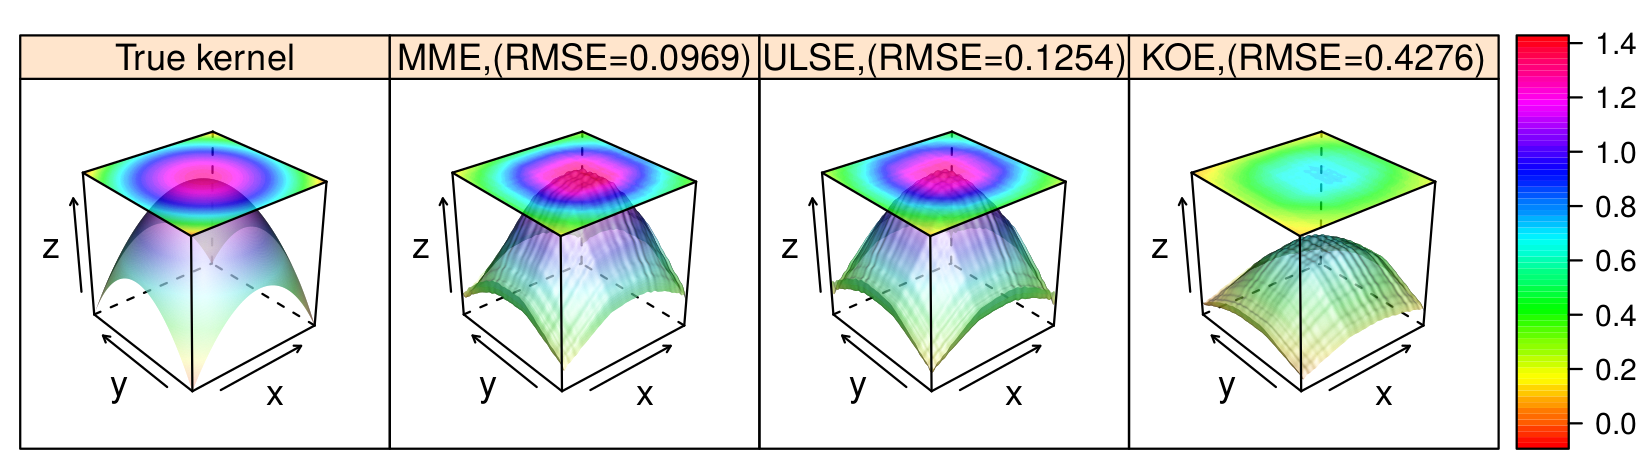
\includegraphics[width=\textwidth]{images/all_methods.png}
\caption{Comparison of all methods of estimations when $n=200$, $\Vert \phi\Vert_\mathcal{S}=0.9$, and $k_n=1$.
\label{fig:compare}}
\end{figure}

\begin{figure}
\centering
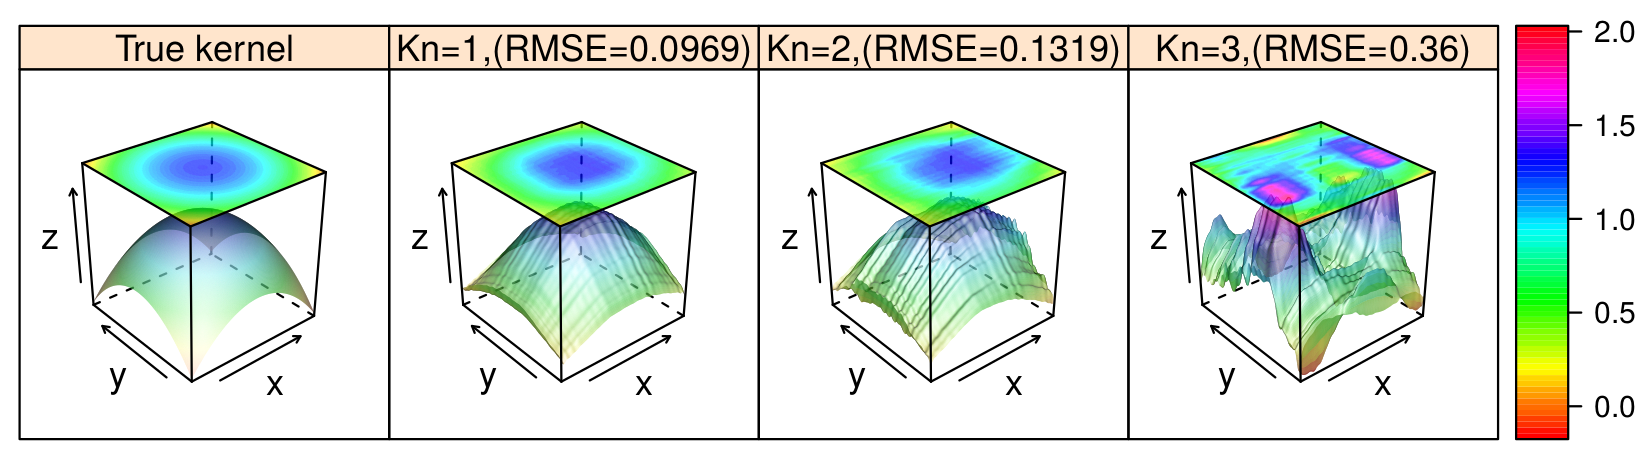
\includegraphics[width=\textwidth]{images/MME.png}
\caption{Method of moment estimation of the model parameter kernel by considering $n=200,\ \Vert \phi\Vert_\mathcal{S}=0.9,$ and $k_n=1, 2, 3.$
\label{fig:mme}}
\end{figure}

\begin{table}
\centering
\resizebox{\columnwidth}{!}{%
\begin{tabular}{ccccccccccccc}
\hline\hline
&&& $\Vert \phi\Vert_\mathcal{S}=0.1$&&&&$\Vert \phi\Vert_\mathcal{S}=0.5$&&&&$\Vert \phi\Vert_\mathcal{S}=0.9$&\\ \cline{3-5}\cline{7-9}\cline{11-13}
n   & $k_n$ & MME    & ULSE   & KOE    & & MME    & ULSE   & KOE    & & MME    & ULSE   & KOE \\ \hline
50  & 1     & 0.1750 & 0.1645 & 0.0951 & & 0.2403 & 0.2838 & 0.3716 & & 0.1986 & 0.2323 & 0.5096\\
    & 2     & 0.5484 & 0.5189 & 0.0959 & & 0.4931 & 0.7000 & 0.3720 & & 0.4387 & 1.0381 & 0.5099\\
    & 3     & 1.0239 & 0.9657 & 0.0961 & & 0.9988 & 1.1478 & 0.3721 & & 1.0435 & 1.7282 & 0.5099\\
    & 4     & 1.5573 & 1.4934 & 0.0962 & & 1.5340 & 1.6513 & 0.3721 & & 1.6382 & 2.4725 & 0.5099\\ \hline
100 & 1     & 0.1222 & 0.1183 & 0.0861 & & 0.2050 & 0.2579 & 0.3539 & & 0.1387 & 0.1709 & 0.4134\\
    & 2     & 0.3662 & 0.3598 & 0.0866 & & 0.3325 & 0.6087 & 0.3541 & & 0.2743 & 0.9728 & 0.4136\\
    & 3     & 0.6830 & 0.6798 & 0.0868 & & 0.6661 & 0.8723 & 0.3541 & & 0.6694 & 1.3925 & 0.4136\\
    & 4     & 1.0645 & 1.0243 & 0.0868 & & 1.0245 & 1.1973 & 0.3542 & & 1.0193 & 1.9377 & 0.4136\\ \hline
150 & 1     & 0.1033 & 0.1027 & 0.0825 & & 0.1946 & 0.2505 & 0.3460 & & 0.1205 & 0.1517 & 0.3735\\
    & 2     & 0.2903 & 0.2900 & 0.0830 & & 0.2666 & 0.5704 & 0.3462 & & 0.2149 & 0.9478 & 0.3737\\
    & 3     & 0.5533 & 0.5449 & 0.0831 & & 0.5387 & 0.7601 & 0.3462 & & 0.5272 & 1.2493 & 0.3736\\
    & 4     & 0.8560 & 0.8237 & 0.0831 & & 0.8256 & 1.0040 & 0.3462 & & 0.8106 & 1.6683 & 0.3736\\ \hline
200 & 1     & 0.0917 & 0.0935 & 0.0798 & & 0.1879 & 0.2457 & 0.3393 & & 0.1114 & 0.1419 & 0.3496\\
    & 2     & 0.2490 & 0.2610 & 0.0803 & & 0.2285 & 0.5568 & 0.3394 & & 0.1818 & 0.9411 & 0.3497\\
    & 3     & 0.4790 & 0.4745 & 0.0804 & & 0.4684 & 0.7047 & 0.3394 & & 0.4542 & 1.1896 & 0.3497\\
    & 4     & 0.7438 & 0.7127 & 0.0804 & & 0.7199 & 0.9042 & 0.3394 & & 0.7040 & 1.5134 & 0.3497\\ \hline
\end{tabular}
} % end of resize
\caption{The NMSE of the parameter estimators. \label{tab: sim}}
\end{table}
%****************************************************************************************************************************

\section{Conclusion}\label{sec:conclusion}

In this paper, we have focused on seasonal functional autoregressive time series. We have presented conditions for the existence of a unique stationary and causal solution. Furthermore, we have derived some basic properties and limiting behaviour. For arbitrary $h\in {\mathbb{N}},$ we have investigated the $h$-step  predictor based on Kargin-Onatski (2008) and Bosq (2014). ****

%****************************************************************************************************************************

\printbibliography

\end{document}
